\section{Diagnosing discrete distributions: Ord plots}%
\label{sec:discrete-Ord}
\ix{Ord plot|(}
Ideally, the general form chosen for a discrete distribution should
be dictated by substantive knowledge of a plausible mechanism
for generating the data.
When such knowledge is lacking, however,
we may not know which distribution is most appropriate for
some particular set of data.
In these cases, the question is often turned around, so that we seek
a distribution that fits well, and then try to understand the mechanism
in terms of aspects of the underlying probability theory (independent trials,
rare events, waiting-time to an occurrence, and so forth).

Although it is possible to fit each of several possibilities,
the summary goodness-of-fit statistics can easily be influenced by
one or two disparate cells, or additional (ignored or unknown) factors.
One simple alternative is a plot suggested by
\citet{Ord:67} which may be used to diagnose
the form of the discrete distribution.  Ord showed that a linear
relationship of the form,
\begin{equation} \label{eq:ord}
  \frac{ k \,  p(k) } { p(k-1) }
 = a  +  b \,  k \comma
\end{equation}
holds for each of the Poisson, binomial, negative binomial, and
logarithmic series distributions, and these distributions are
distinguished by the signs of the intercept,
$a$, and slope, $b$, as shown in
\tabref{tab:ordparm}.
The slope, \(b\),
in \eqref{eq:ord} is zero for the
Poisson, negative for the binomial, and positive for the negative
binomial and logarithmic series distributions; the latter two are
distinguished by their intercepts.
\ix{Poisson distribution}
\ix{logarithmic series distribution}
\ix{binomial distribution}
\ix{negative binomial distribution}

Thus, a plot of \(k \,  n_k /  n_{k-1}\) against \(k\), if linear,
is suggested as a means to determine which of these distributions to apply.
The values of the slope and intercept provide rough estimates of the
distribution parameters.

\begin{table}[htb]
\caption[Diagnostic slope and intercept for four discrete distributions]{Diagnostic slope and
intercept for four discrete distributions.  The ratios $k n_k / n_{k-1}$ plotted
against $k$ should appear as a straight line, whose slope and intercept
determine the particular distribution.}
\label{tab:ordparm}
\begin{center}
%\vspace{1ex}
\begin{tabular}{|ccll|}\hline
Slope & Intercept & Distribution & Parameter \\
(b)   & (a)       & (parameter)  &  estimate \\ \hline
0     &  $+$      &  Poisson (\(\lambda\)) & \(\lambda = a\)    \\
$-$   &  $+$      &  Binomial (n, p)       & \(p = b / (b-1)\)  \\
$+$   &  $+$      &  Negative binomial (n,p)      & \(p = 1 - b\)      \\
$+$   &  $-$      &  Log.\ series (\(\theta\)) & \(\theta =  b\) \\
      &      &                     &   \(\theta = - a\) \\ \hline
\end{tabular}
\end{center}
\end{table}

\subsubsection{Fitting the line}
One difficulty in applying this technique is that the number of points
(distinct values of $k$)
in the Ord plot is often small, and the sampling variances of
\(k \,  n_k /  n_{k-1}\) can vary enormously.
A little reflection indicates that points where $n_k$ is small
should be given less weight in determining the slope of the
line (and hence determining the form of the distribution).
In the small number of cases I've
tried, I have found that using a weighted least squares fit of \(k \,
n_k /  n_{k-1}\) on \(k\), using weights of \(w_k = \sqrt { n_k -1
}\)
produces reasonably good%
\footnote{This definition implies that frequencies of $n_k =1$
are ignored in fitting the line.}
automatic diagnosis of the form of a
probability distribution, but this choice is surely open to further study.

\subsubsection{Examples}
\begin{Example}[horskick3]{Death by horse kick}
The table below shows the calculations for
the horse kicks data, with the ratio \({ k \,  n_k } /  { n_{k-1}
}\) labeled \texttt{y}.  The weighted least squares line, with weights
\(w_k\), has a slope close to zero, indicating the Poisson
distribution.  The estimate \(\lambda = a = .656\) compares
favorably with the MLE, $\lambda=0.610$ and the
value from the Poissonness plot, shown in the
following section.
\ixd{death by horse kick}

\begin{alltt}
      Ord Plot: Deaths by Horsekicks

   k     \(n\sb{k}\)    \(n\sb{k-1}\)       \(w\sb{k}\)         y

   0    109      .    10.3923     .        -- Weighted LS --
   1     65    109     8.0000    0.5963    slope = -0.034
   2     22     65     4.5826    0.6769    inter = 0.656
   3      3     22     1.4142    0.4091
   4      1      3     0.0000    1.3333
\end{alltt}
\end{Example}

\begin{Example}[madison3]{Federalist papers}
For the word frequency data, the slope is positive, so either the
negative binomial or log series are possible.  The intercept is
essentially zero, which is ambiguous.  However, the logarithmic
series requires \(b \approx  - a\), so the negative binomial is a
better choice.  Mosteller \& Wallace did in fact find a reasonably
good fit to this distribution.
\ix{logarithmic series distribution}
\ix{negative binomial distribution}
\ixd{Federalist papers}

\begin{alltt}
      Instances of 'may' in Federalist papers

   k     \(n\sb{k}\)    \(n\sb{k-1}\)       \(w\sb{k}\)         y

   0    156      .    12.4499     .       -- Weighted LS --
   1     63    156     7.8740    0.4038   slope = 0.424
   2     29     63     5.2915    0.9206   inter = -0.023
   3      8     29     2.6458    0.8276
   4      4      8     1.7321    2.0000
   5      1      4     0.0000    1.2500
   6      1      1     0.0000    6.0000
\end{alltt}

Plots of data fitting four different discrete distributions are
shown in \figref{fig:orddemo}, using the data previously examined
in this chapter.
In each case, the slope and intercept of the weighted least squares line correctly
identify the distribution.
\end{Example}

\subsubsection{Drawbacks}
Using a single plot to determine one of four common discrete
distributions is advantageous, but our enthusiasm should be
limited by several weaknesses:

\begin{itemize*}
\item The Ord plot lacks resistance, since a single discrepant
       frequency affects the points for both \(k\) and \(k  +  1\).

\item The sampling variance of \(k \,  n_k /  n_{k-1}\) fluctuates
       widely
       \citep{HoaglinTukey:85,JinkinsonSlater:81}.  The use of weights \(w_k\) helps, but is purely a
       heuristic device.
\end{itemize*}


\begin{figure}[htb]
 \begin{minipage}[b]{.5\linewidth}
  \centering
  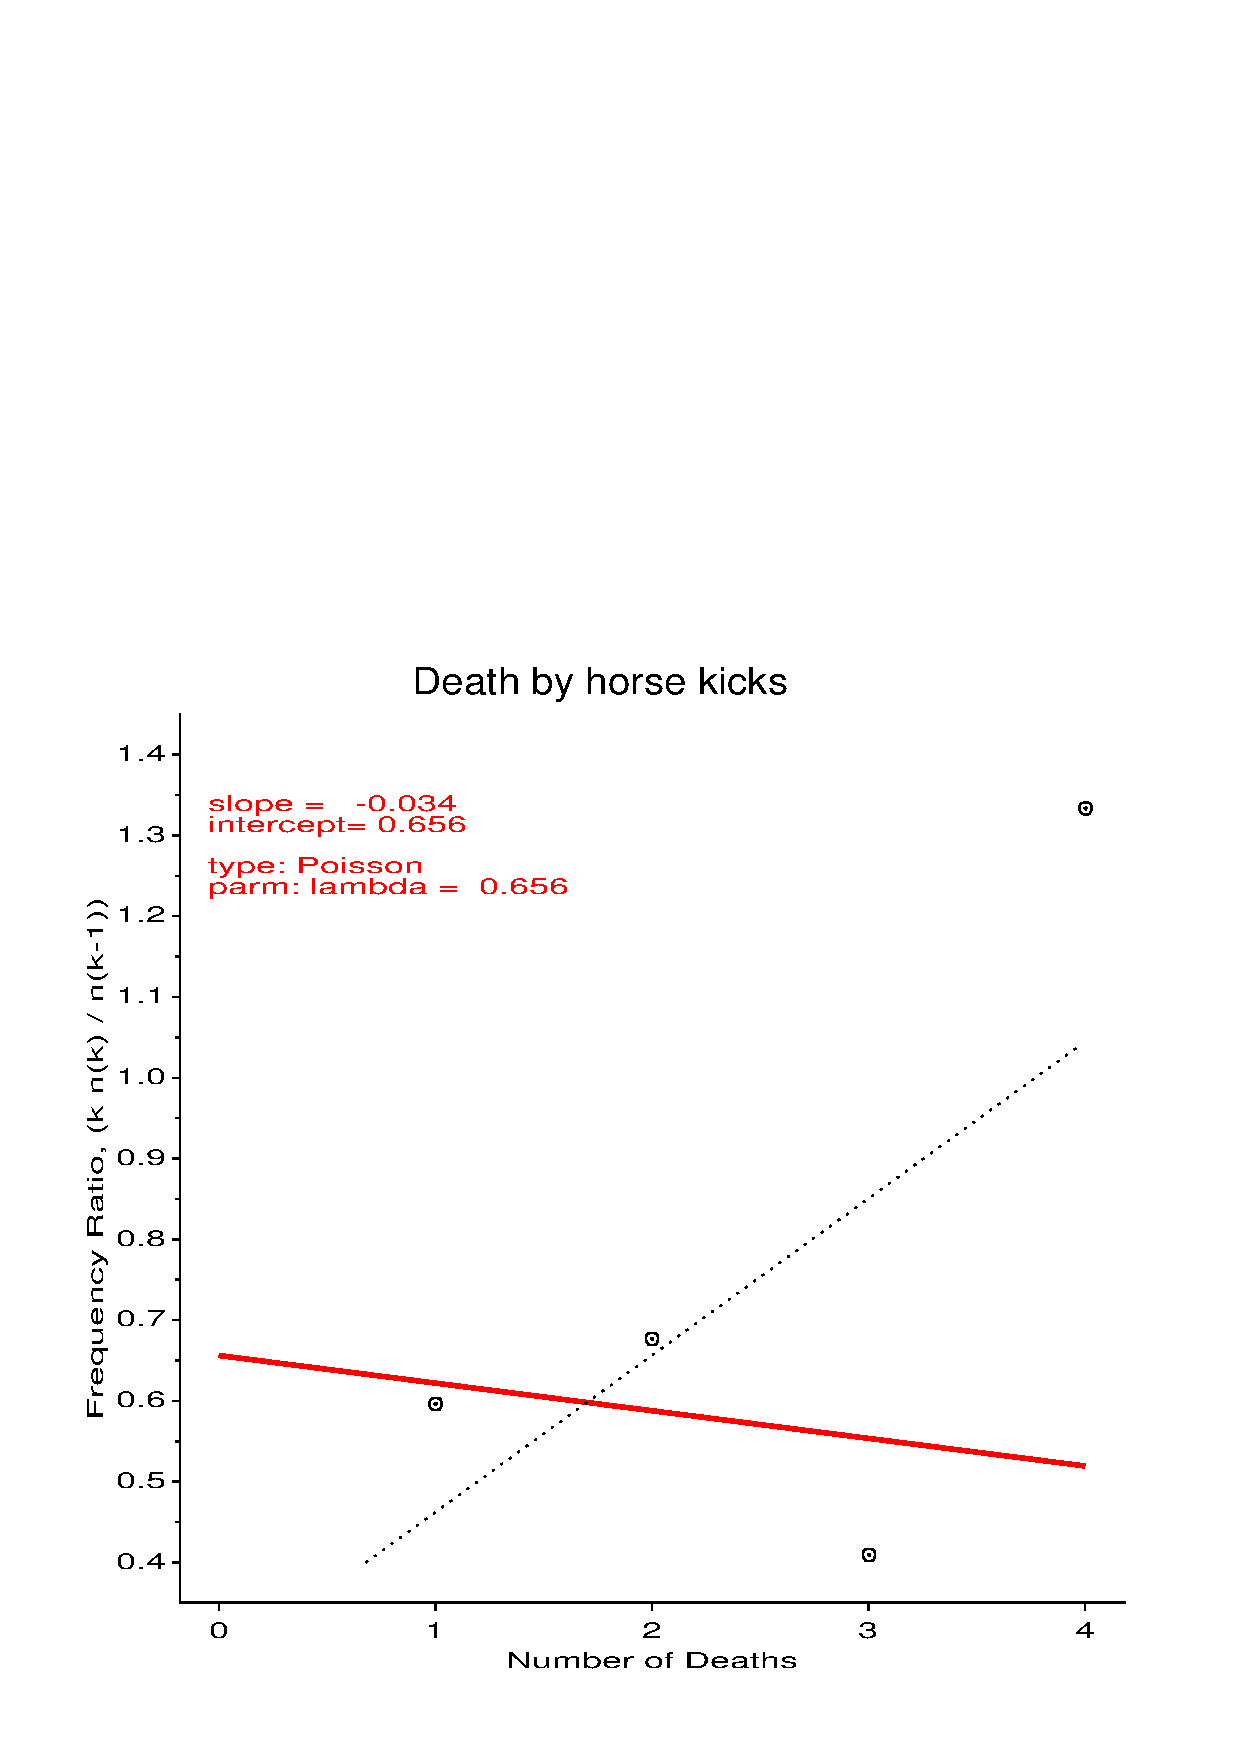
\includegraphics[width=.9\linewidth]{orddemo1}\graphicsfile{ch2/fig/orddemo1.eps}{}
 \end{minipage}%
 \begin{minipage}[b]{.5\linewidth}
  \centering
  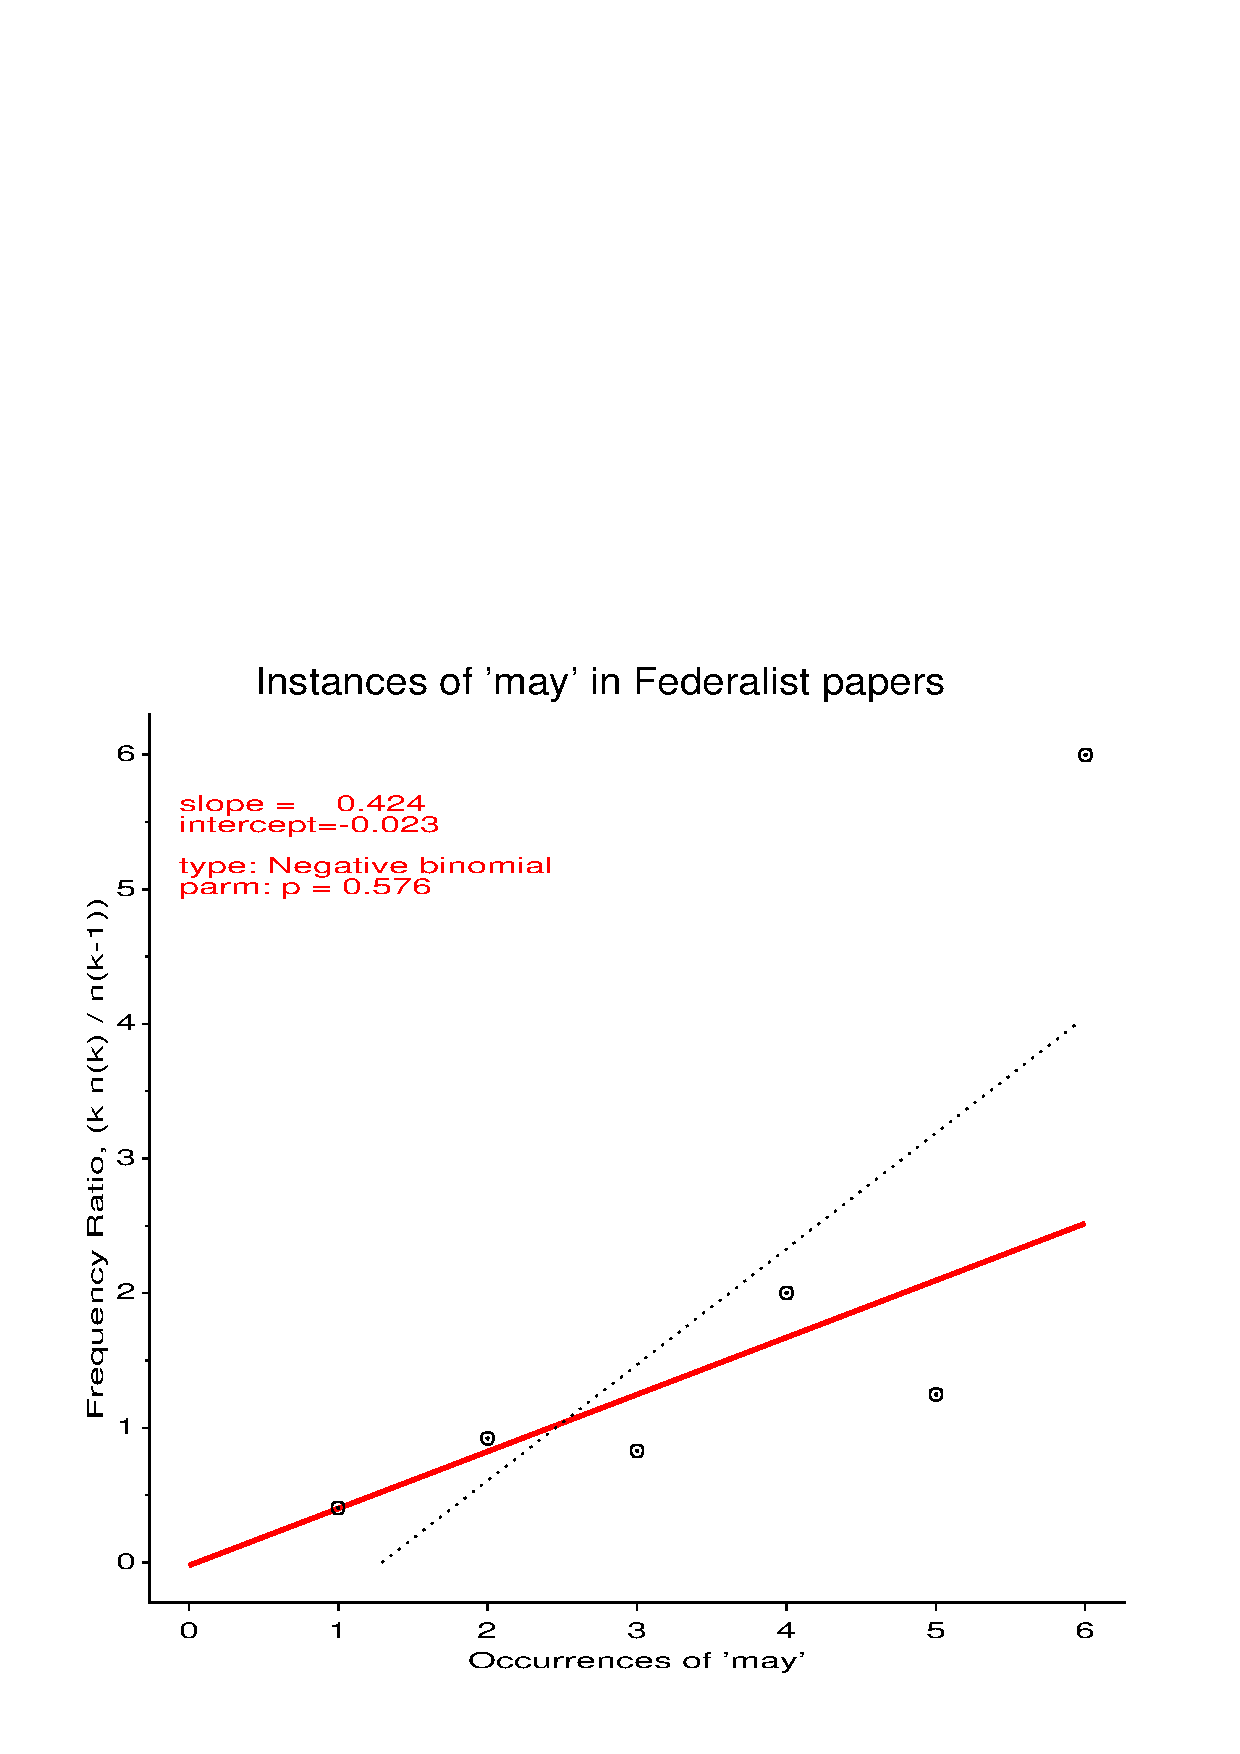
\includegraphics[width=.9\linewidth]{orddemo2}\graphicsfile{ch2/fig/orddemo2.eps}{}
 \end{minipage}
 \\[3ex]
 \begin{minipage}[b]{.5\linewidth}
  \centering
  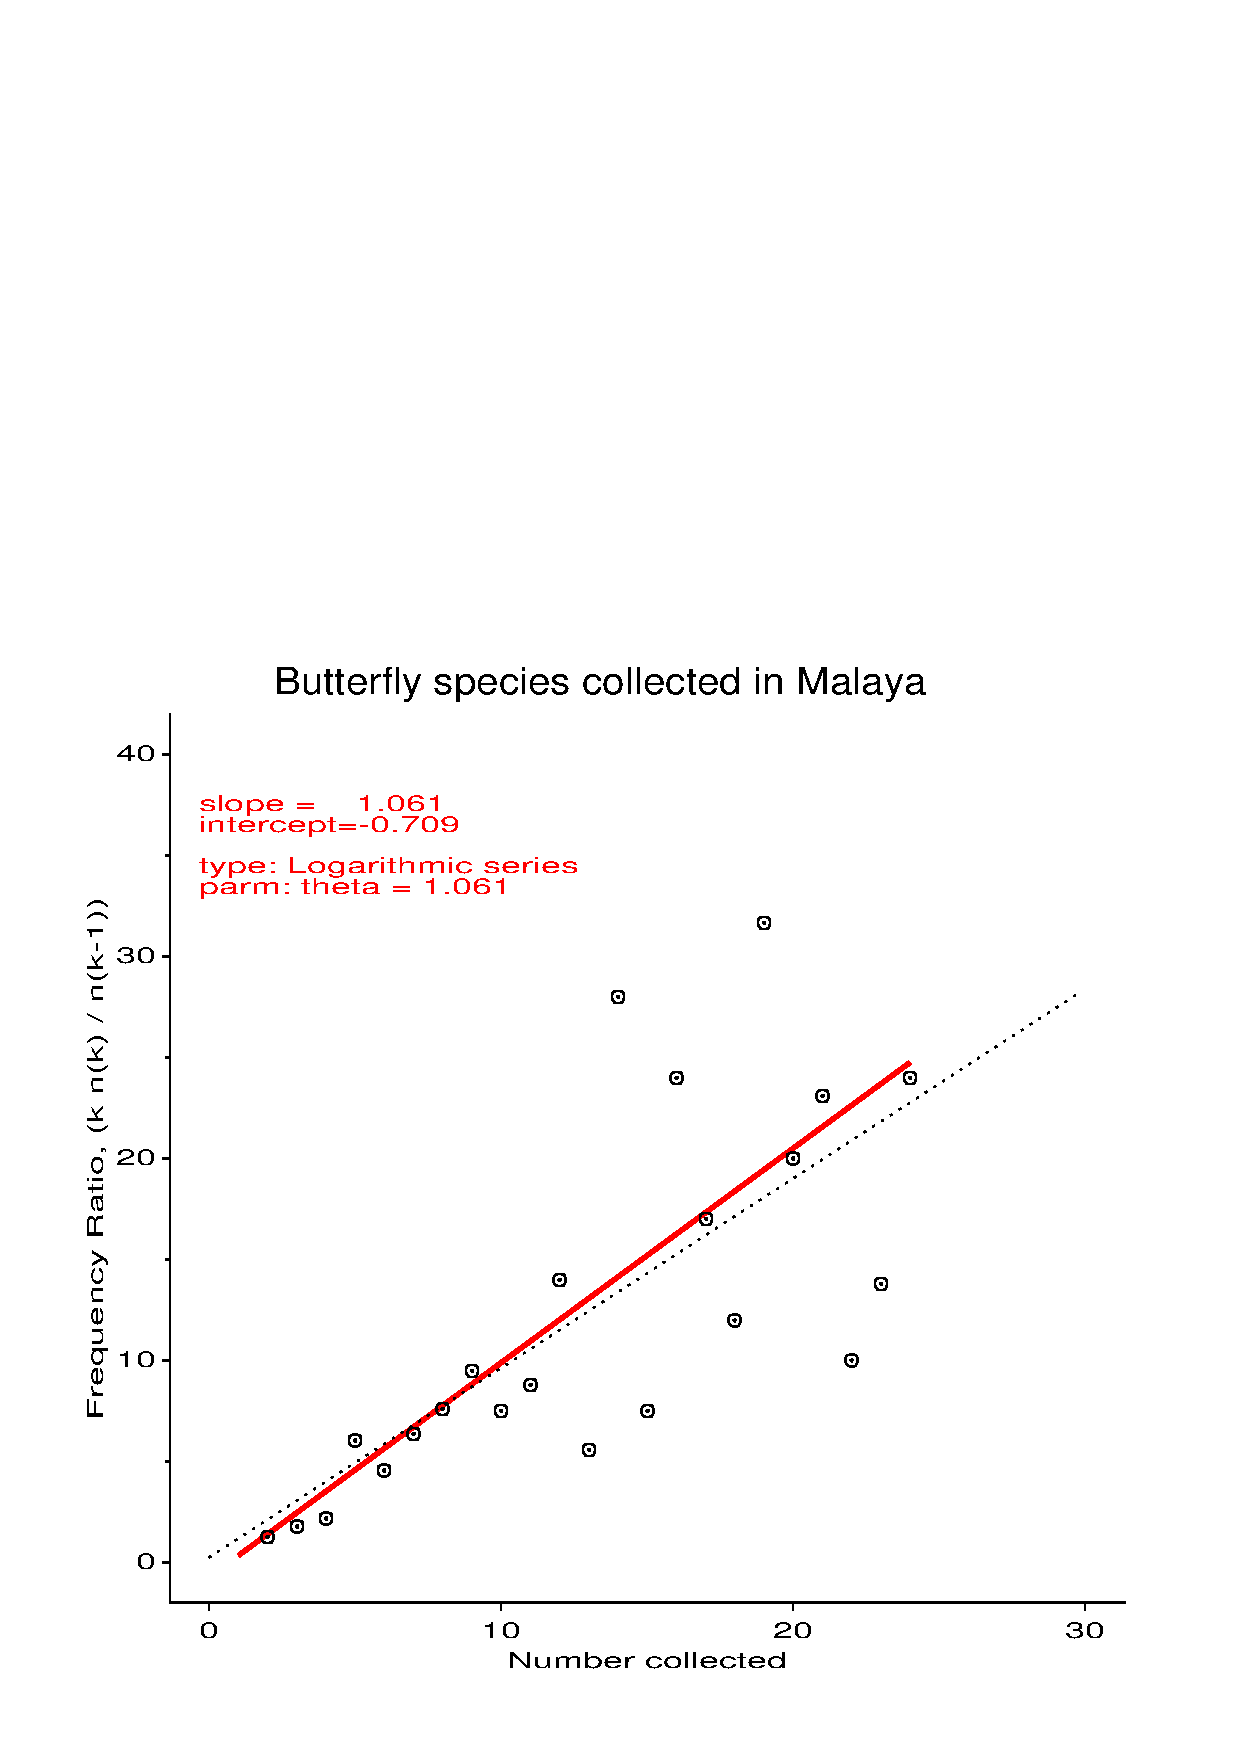
\includegraphics[width=.9\linewidth]{orddemo3}\graphicsfile{ch2/fig/orddemo3.eps}{}
 \end{minipage}%
 \begin{minipage}[b]{.5\linewidth}
  \centering
  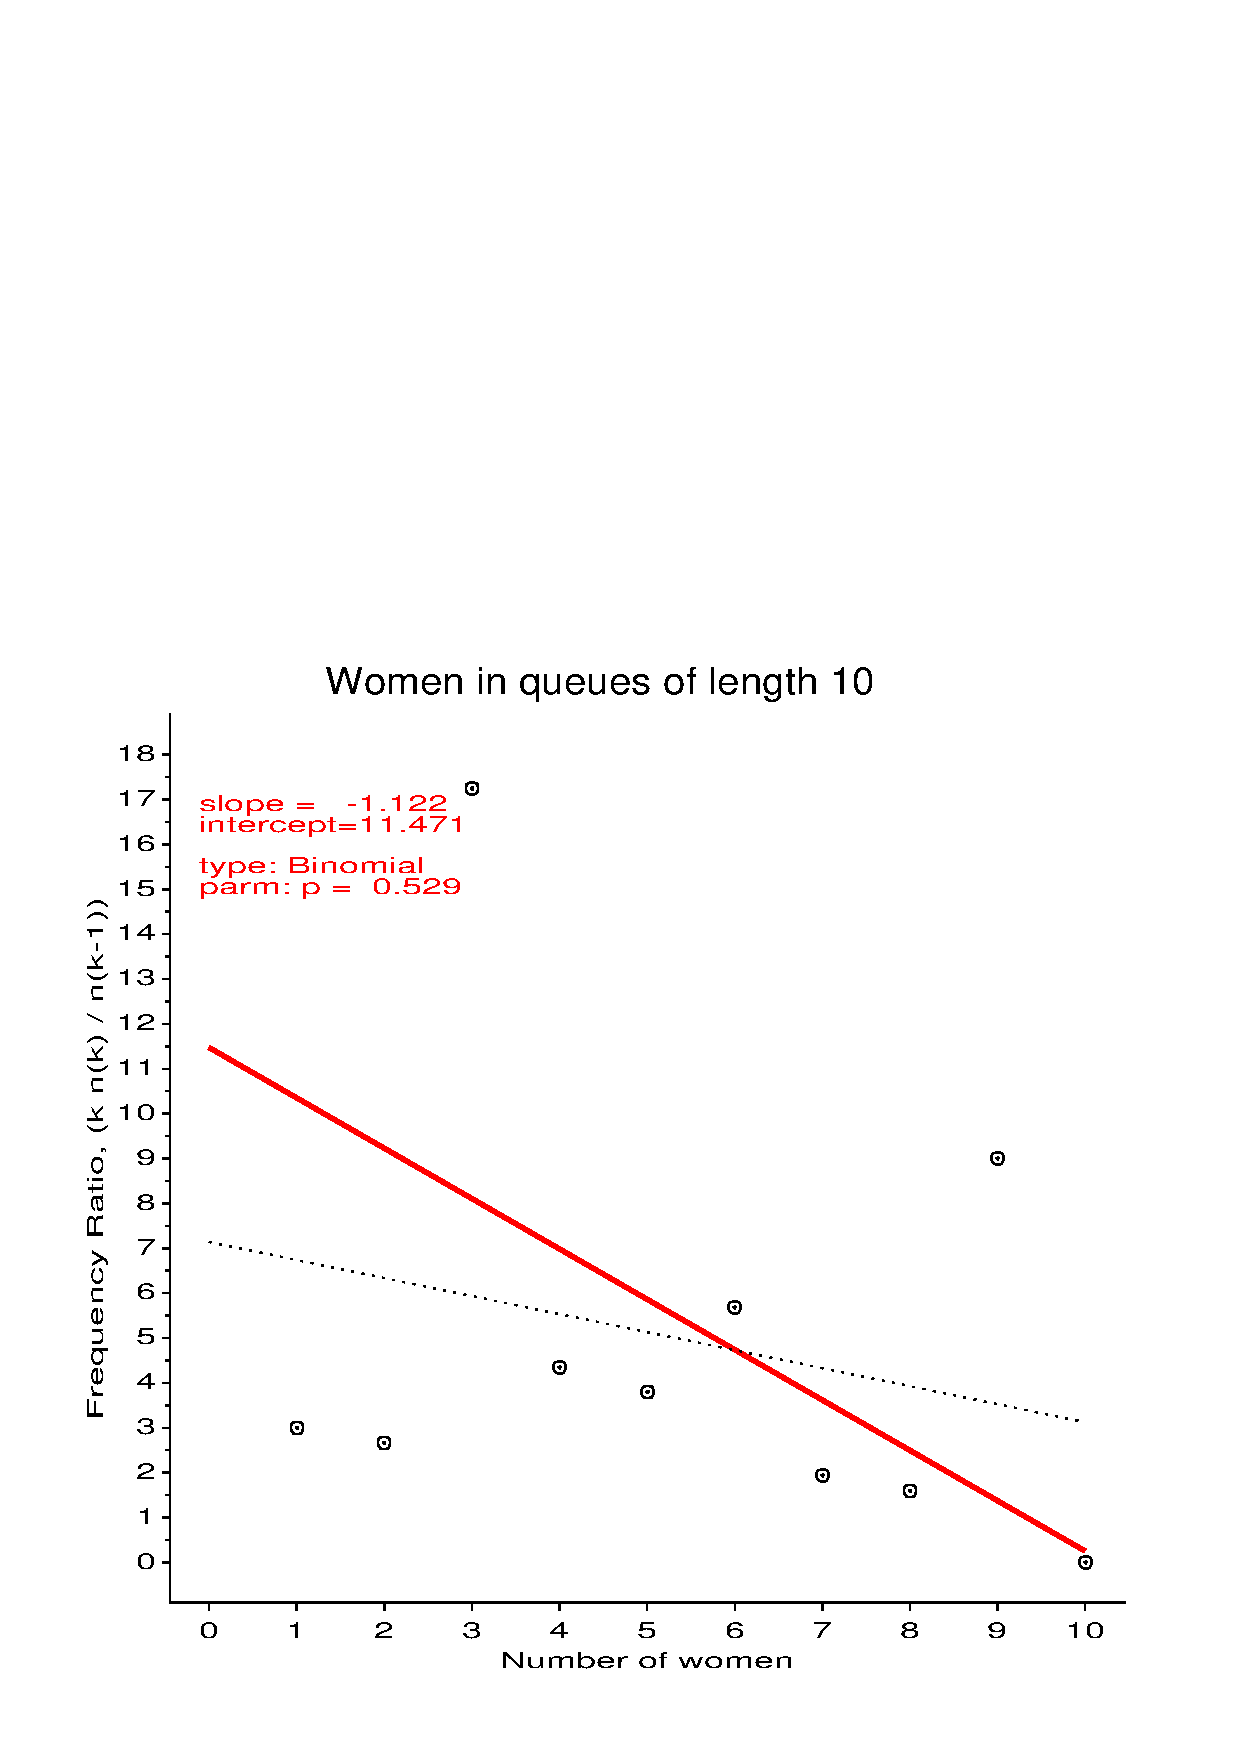
\includegraphics[width=.9\linewidth]{orddemo4}\graphicsfile{ch2/fig/orddemo4.eps}{}
 \end{minipage}
 \caption[Ord plots for four discrete distributions]{Ord plots for four discrete
distributions.  Each panel shows the least squares line (dotted, black) and the weighted least squares line (solid, red). The slope and intercept of the weighted least squares line are used to
identify the type of the distribution.}\label{fig:orddemo}
\end{figure}

\subsubsection{ORDPLOT macro}
These plots are produced by the \macro{ORDPLOT} (see \ref{mac:ordplot}).  For the horse kicks
data,  the plot in \figref{fig:orddemo} is produced with the macro call
\begin{listing}
%ordplot(data=horskick,
         count=Deaths, freq=corpsyrs);
\end{listing}
The \mparm{FREQ}{ORDPLOT} gives the name of the basic frequency variable ($k$),
and the \mparm{COUNT}{ORDPLOT} gives the associated count, $n_k$.
\ix{Ord plot|)}
